\section{Introduction}

  \subsection{Field Programmable Gate Arrays}

    \underline{F}ield \underline{P}rogrammable \underline{G}ate \underline{A}rrays (FPGAs) are silicon based integrated circuit chips.
    Unlike conventional chips, where the circuit and logic gates are permanently synthesized from silicon transistors at manufacture time, the internal structure of an FPGA can be manipulated to the desired structure of the user.
    The advantage of FPGAs is the high data transfer rates and versatility they deliver, without the cost of manufacturing purpose built chips. 
    As such, FPGAs are used extensively in the development of new technology and small batch size production. \cite{fpga}
    \par
    FPGAs are programmed in a variety of languages known as \underline{H}ardware \underline{D}escription \underline{L}anguages (HDLs).
    One of the more common HDLs and the HDL used in this project is \underline{V}ery High Speed Integrated Circuit \underline{H}ardware \underline{D}escription \underline{L}anguages (VHDL).
    Programing a circuit in VHDL requires the creation of entities, sometimes refereed to as modules.
    These entities can be thought of as a \textit{`black boxes'} that compute logic on their inputs and thus form their outputs.
    The form of this logic computed by the entity is known as the entities' architecture.
    \par
    When building a circuit larger than one simple function it is often necessary to use more than one entity.
    In VHDL entities can contain sub-entities within their architecture; entities that do this are known as top-level entities.
    Top level entities are often used to commute signals between there sub-entities and/or control how sub-entities operate.

	\subsection{The Standard Model of Particle Physics}

    Central to the modern study of particle physics is the standard model,
    % \vspace{-0.1em}
    \begin{multline} \label{eqn:std-mod}
      L_{GWL} = \sum_{f} ( \bar{\Psi}_{f} ( i \gamma^\mu \partial \mu - m_{f} ) \Psi_{f} - eQ_{f} \bar{\Psi}_{f} \gamma^\mu \Psi_{f} A_{\mu} ) + \frac{g}{\sqrt{2}} \sum_{i} ( \bar{a}^i_L \gamma^\mu b^i_L W^+_\mu + \bar{b}^i_L \gamma^\mu a^i_L W^-_\mu )                        \\                           
              + \frac{g}{2x_w} \sum_f \bar{\Psi}_f \gamma^\mu ( I^3_f - 2s^2_w Q_f - I6e_f \gamma_5 ) \Psi_f Z_\mu - \frac{1}{4} | \partial_\mu A_v - \partial_v A_\mu - ie(W^-_\mu W^+_v - W^+_\mu W^-_v ) |^2                                         \\                                     
              - \frac{1}{2} | \partial_\mu W^+_v - \partial_v W^+_\mu - ie ( W^+_\mu A_v - W^+_v A_\mu ) + ig' c_w (W^+_\mu Z_v - W^+_v Z_\mu |^2 \\
              - \frac{1}{4} | \partial_\mu Z_v - \partial_v Z_\mu + ig' c_w (W^-_\mu W^+_v - W^+_\mu W^-_v ) |^2 - \frac{1}{2} M^2_\eta \eta^2  - \frac{gM^2_\eta}{8M_W} \eta^3  - \frac{g'^2 M^2_\eta}{32M_W}\eta^4    \\     
              + | M_W W^+_\mu + \frac{g}{2} \eta W^+_\mu |^2 + \frac{1}{2} | \partial_\mu \eta + i M_Z Z_\mu + \frac{ig}{2c_w} \eta Z_\mu |^2 - \sum_f \frac{g m_f}{2 M_W} \bar{\Psi}_f \Psi_f\ \eta. 
              \vspace{1em}                                                                               
    \end{multline}
    % \vspace{0.5em}
    The standard model shown in equation \ref{eqn:std-mod}, is a quantum field theory that describes the fundamental particles and how they interact.
    While this document does not require or attempt a detailed understanding of the intricate detail of the standard model,
    the aim of many particle physics experiments is to verify, measure and expand the model.
    Despite being the current best theory to explain particle interactions, the model is not complete.
    There are many un-described phenomena, such as the matter domination in the universe, that require physics beyond the standard model in order to be described.
    To that end, major international efforts, namely in the form of the Large Hadron Collider, aim to gain further knowledge and understanding of the underlying physics of the universe. \cite{ref:std}

  \subsection{The LHCb Experiment}

    One experiment at the Large Hadron Collider is Large Hadron Collider beauty (LHCb).
    Located at intersection point 8, LHCb is designed to study rare particle physics phenomena, such as lepton flavor violation and CP violation. 
    LCHb studies the decay modes of the B meson.
    These hadrons travel on the order of $\mu m$s in the detector before decaying. 
    As such, B meson decays can be identified by decay products that propagate from a secondary vertex.

    \begin{figure}[h!]
      \centering
      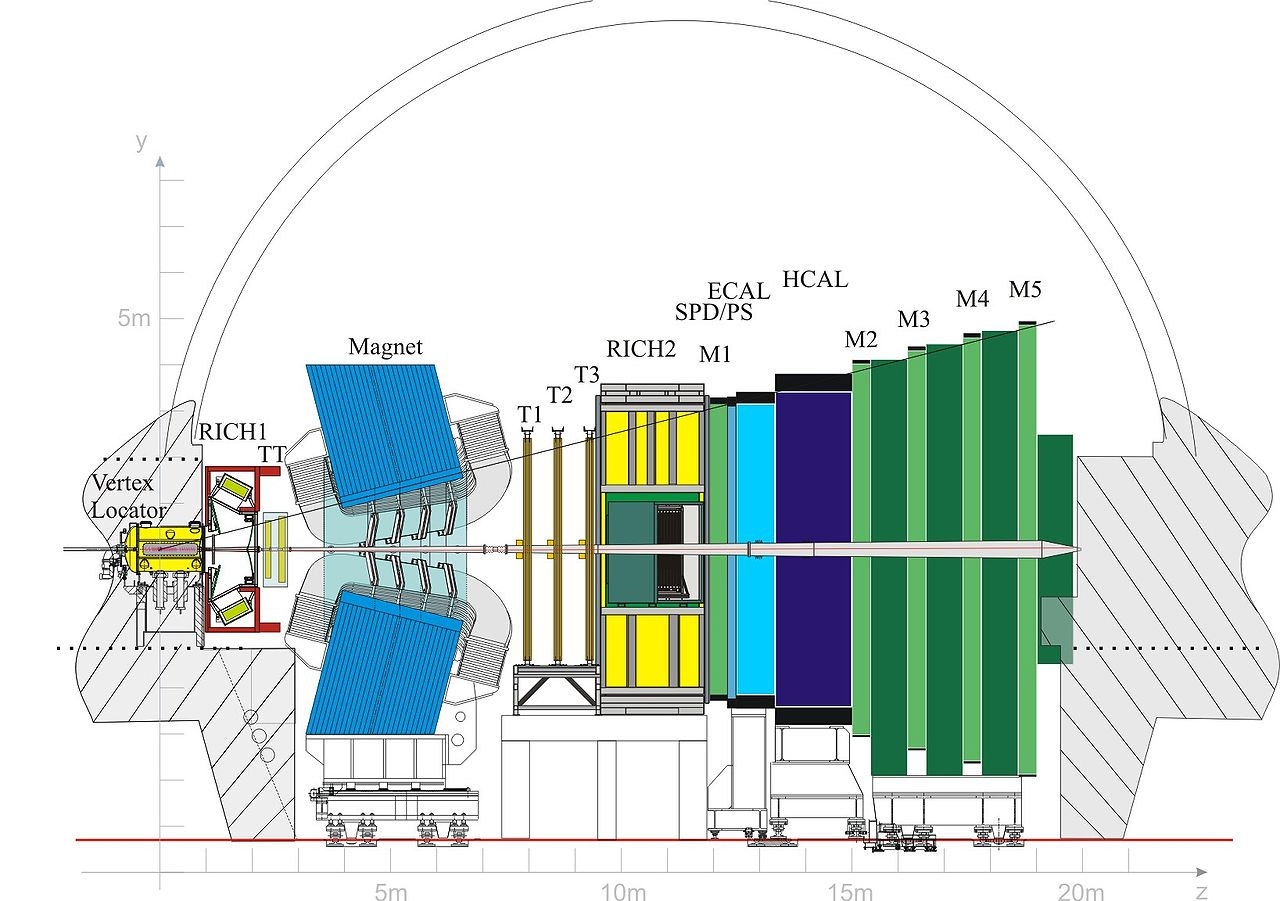
\includegraphics[scale=0.5]{LHCb_Det.jpg}
      \caption{The LHCb Detector along the bending plane.}
      \label{fig:LHCb_Collab}
    \end{figure}

    As B mesons are light (in comparison to many other particles studied in the LHC), the decay products are produced at a shallow angle relative to the beam pipe;
    this is the driving factor in the design of the experiment. 
    LHCb is a single arm forward spectrometer.
    Surrounding the point of collision is the \underline{Ve}rtex \underline{Lo}cator (VELO), this high precision detector uses silicon strips to detect ionising particles as they propagate from a collision and provides the coordinates of the particle in terms of R\footnote{Radial distance from the beam pipe.} and $\phi$\footnote{Azimuthal angle from the beam pipe.}.
    By reconstructing the paths of particles back to the intersection point, it can be identified whether the particular decay particles are a product of the primary vertex\footnote{The position at which the protons collided.}, or a secondary vertex\footnote{The decay point of a short lived particle. i.e. B Meson.}.
    \par
    The RICH detector, comprised of two sub detectors located either side of the magnet, uses Cherenkov radiation to deduce the velocity of the particle. The silicon trackers, labeled TT and T1-3 in Figure~\ref{fig:LHCb_Collab}, calculate the angle deflection by the magnet. 
    By combining the velocity and angle of deflection, the mass, momentum and energy of the particles can be deduced from simple relativistic kinematics,
    \begin{equation}
      E^2 = M^2c^4 + p^2c^2.
    \end{equation}
    The Muon detectors, labeled M1-5 in Figure~\ref{fig:LHCb_Collab}, are designed to detect muon's the detector. 
    This is of particular importance in LHCb as Muons can be easily misidentified as charged Pions, due to their similar mass.
    Pions and Muons are a common decay product of the interactions studied at LHCb, furthering the need to accurately differentiate Muons and Pions.
    \par
    HCAL and ECAL, shown in Figure~\ref{fig:LHCb_Collab}, are hadronic and electric calorimeters respectively. 
    Both measure the total energy of incoming particles.
    As the calorimeters absorb the particles they detect, any leptonic particle reaching the M2-5 muon detectors can be assumed to be a muon.

  \subsection{LHCb Upgrade} % (fold)
  \label{sub:lhcb_upgrade}

    With advancements in accelerator technology, the detectors must also advance in order to make best use of the accelerators.
    The LHC is scheduling to increase its luminosity during \underline{L}ong \underline{S}hutdown \underline{2} (LS2), and as such LHCb will have to cope with this greater luminosity.
    The front end electronics of LHCb implement a hardware trigger (later followed by a software trigger) and this is limited to a 1MHz maximum readout speed.
    Post LS2, LHCb will have to cope at a luminosity of $\mathcal{L} = 2.10^{33} cm^{-2}s^{-1}$; this is significantly greater than the current $\mathcal{L} = 4.10^{32} cm^{-2}s^{-1}$.
    A simple luminosity increase will not significantly reduce the uncertainty for some statistical error dominated channels.
    To achieve greater statistical significance, greater resolution of the VELO and a fully software based trigger is required.
    Detailed in the \textit{`LHCb VELO Upgrade Technical Design Report'} \cite{velo_design_report} the main goals of the 2019 upgrade are as follows:

    \begin{easylist}[itemize]
      & Increase the luminosity to $\mathcal{L} = 2.10^{33} cm^{-2}s^{-1}$.
      & Read data from the detector at the bunch crossing frequency, 40 Mhz.
      & Convert to a purely software based trigger.
    \end{easylist}

    % subsection lhcb_upgrade (end)

    \subsubsection{VELO Upgrade}

      Common with its predecessor, the upgraded VELO uses thin, retractable modules.
      The advantage of this approach is that during collisions, the modules can sit closer than otherwise possible to the beam line.
      The modules retract for the beam fill, avoiding the radiation damage from the wider fill beams.
      In order to gain greater resolution of secondary vertices's, the upgraded VELO will sit at $5.1$ mm from the beam at the closest pixel \cite{velo_design_report}.
      The current VELO achieves 8 mm \cite{velo_web}.
      
      \begin{figure}[ht]
        \centering
        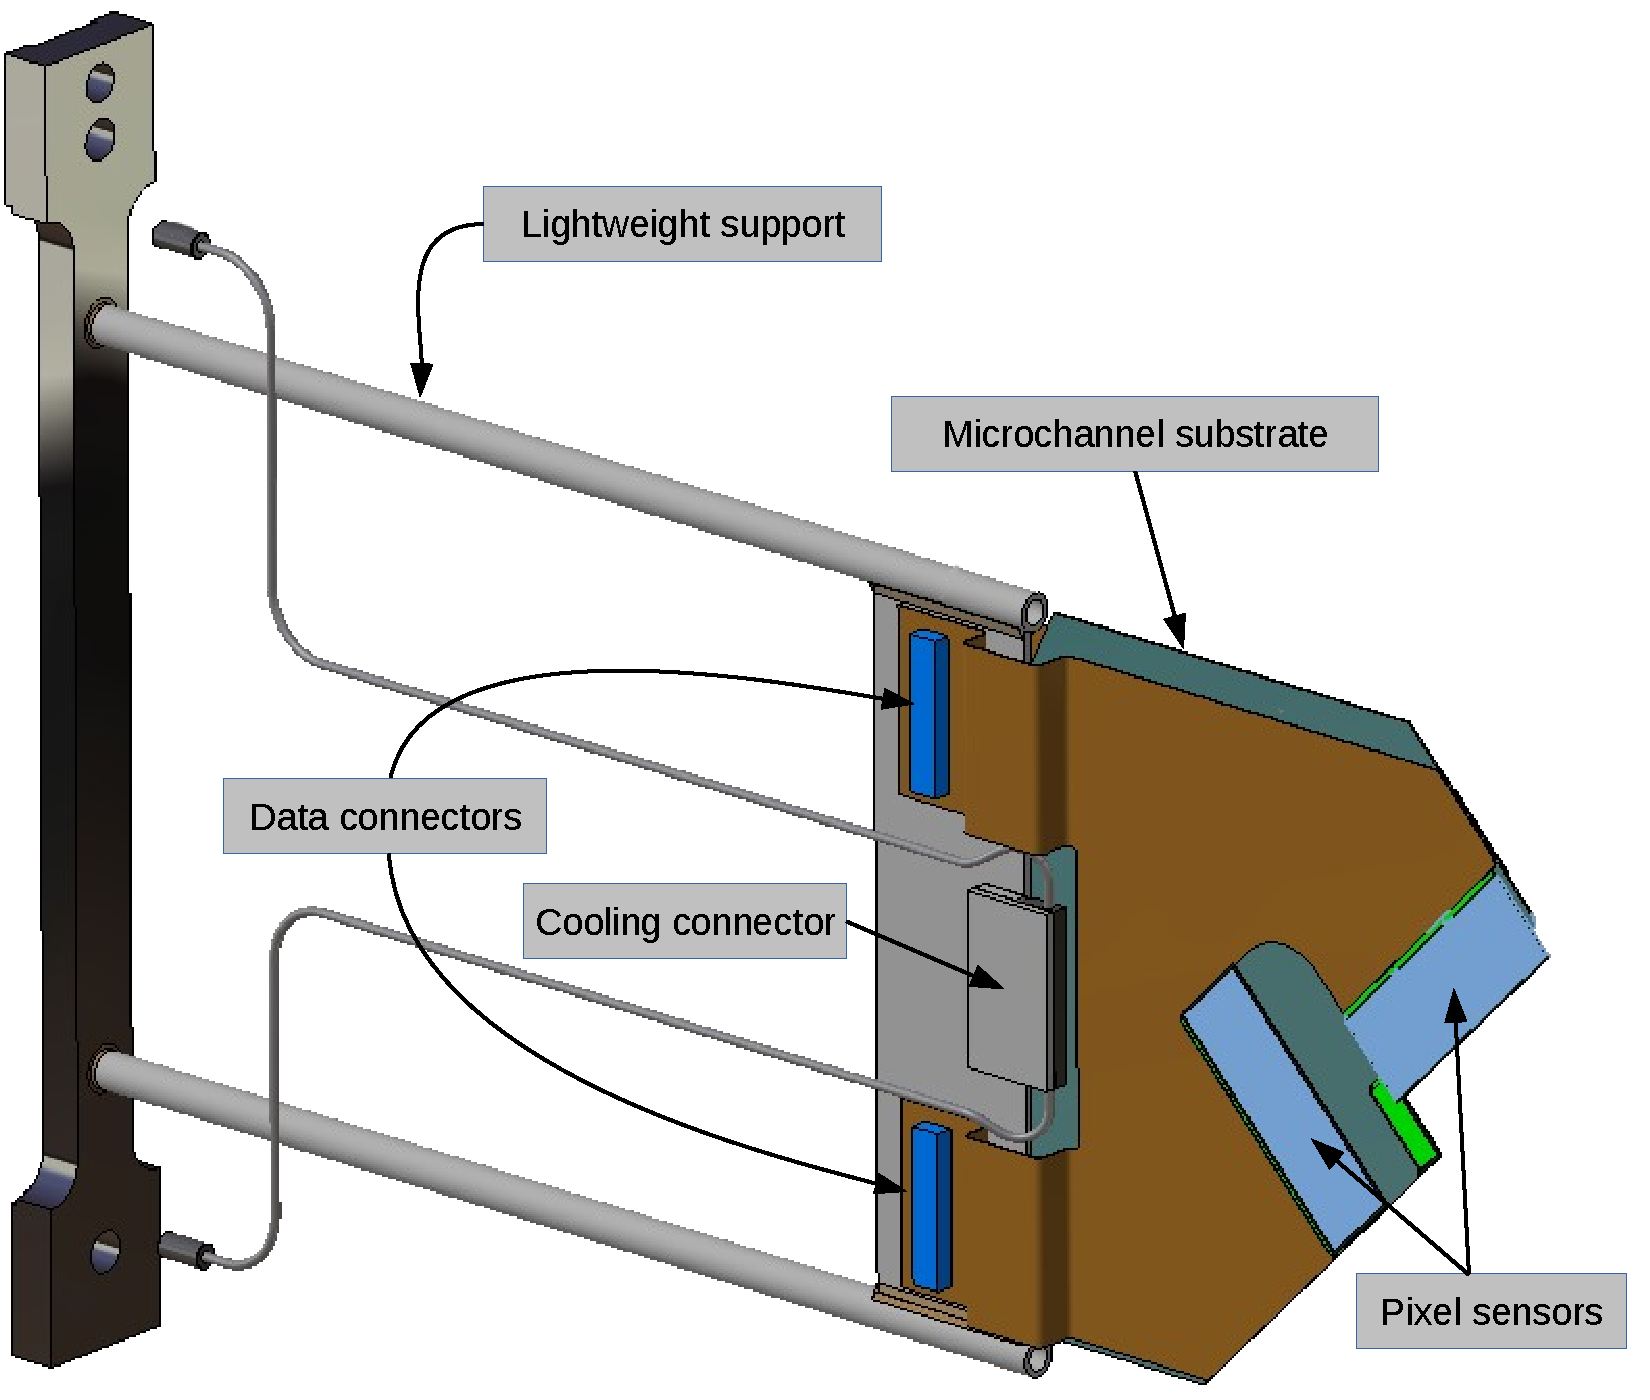
\includegraphics[width=0.75\textwidth]{module}
        \caption{The current module design. Two sensors are shown, the remaining two are mounted to the rear face of the module to form two horizontal rows - covering the rightmost area of the module (as viewed in the figure).}
        \label{fig:module}
      \end{figure}

      As previously mentioned, the current VELO uses silicon strips to detect particles.
      The upgraded VELO, however, will use silicon pixels.
      These pixels, $55 \mu m \times 55 \mu m$ in size and $200 \mu m$ thick \cite{velo_design_report}, are arranged in a 256 wide square matrix on a ASIC chip.
      The pixels are arranged into groups of 8 to form a \underline{S}uper \underline{P}ixel (SP).
      The ASIC chips are arranged in a row of 3 and bonded to a sensor.
      Each module has 4 sensors, 2 per side, as shown in Figure~\ref{fig:module}. 
      The module is cooled by bi-phase CO$_2$ in micro-channels etched into the micro channel substrate. \cite{velo_design_report}
      \par
      The VELO modules will operate in the LHC secondary vacuum.
      It is separated from the primary vacuum by RF foil that is 3.5mm from the beam-line, at the closest point \cite{velo_design_report}.
      The foil is made of 250 $\mu m$ thick aluminum to reduce its interaction with the collision decay products. 

      \subsubsection{Data Flow and Low Level Interface}   

      FPGAs are used in the \underline{D}ata \underline{A}c\underline{q}uisition (DAQ) modules for their speed and parallel processing capabilities.
      The DAQ, in its simplest form, is a series of optical links, a data processing FPGA and a PCIe port for data transfer to the VELO computer system.
      \par
      The data from each SP is packaged in a 30 bit \underline{S}uper \underline{P}ixel \underline{P}acket (SPP). The SPP is comprised of  a (from most to least significant bits) 9 bit \underline{B}unch \underline{C}ross \underline{ID} (BCID); 13 bit SPP location information (horizontal and vertical coordinates); 8 bit SP hit map.
      \par
      A GWT serialiser in the ASIC forms a 128 bit \textit{`frame'} comprising of a header (1010), four single bit parity flags and four SPPs.
      The parity flags indicate the parity of the four SPPs as a validation check for downstream processes.
      The data is then transmitted via an electrical to optical converter though optical fibers to the DAQ.
      \begin{figure}[ht]
        \centering
        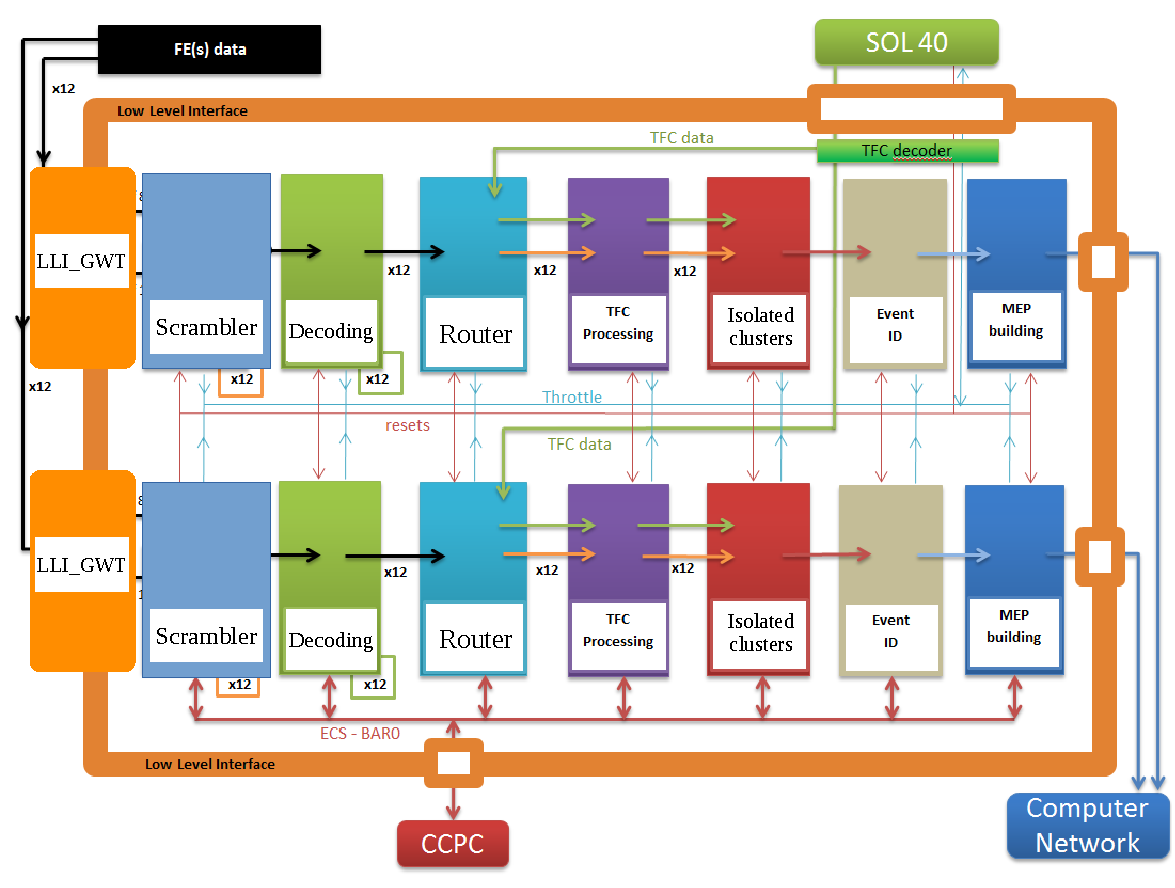
\includegraphics[width=\textwidth]{low_level_interface}
        \caption{A Diagram showing the data flow in the low level interface.}
        \label{fig:lli}
      \end{figure}
      Located on the DAQ FPGA is the \underline{L}ow \underline{L}evel \underline{I}nterface (LLI).
      The LLI is responsible for sorting the incoming data into time order and packaging the data in the correct form for the computer systems and to optimise output bandwidth.
      Other processes included in the LLI are descrambling and event isolation tagging.
      These processes will be discussed in more detail later in this document.
